\usepackage{../submodules/FancyBeamer/fancybeamer} % use the fancy beamer package
%\fancylogos{,uulm,,unibe,,ovgu-blue,}
\setfancycolumnsdefault{animation=keep} % animate all columns per default

% GRAPHICSPATH

\setpaths{
	{../pics/}
}

% IMPORTED PACKAGES

\usepackage{multicol} % used temporarily for the lecture overview
\usepackage{stmaryrd} % \lightning in modeling lecture
\usepackage{catchfile} % read picture sources from files
\usepackage{silence} % ignore some warnings
\WarningFilter{latex}{You have requested package} % ignore warning for loading packages from submodules
%\usepackage{../EagleoutIce-fancyqr/fancyqr} % QR codes for practice task, credits to Florian Sihler
\usepackage{fancyqr} % QR codes for practice task, credits to Florian Sihler
\fancyqrset{gradient=true,gradient angle=-45,l color=black,r color=blue}
\usepackage{ifthen} % \ifuniversity
\usepackage{booktabs} % tables
%\usepackage{colortbl} % \rowcolor used in Lecture 8 in SPL
%\usepackage{algpseudocode} % used in Lecture 10 in SPL

% INCLUDED TEMPLATE FILES

% TYPICAL COMMANDS FOR LECTURES

\renewcommand{\emph}[1]{{\color{blue}\textbf{#1}}}
%\ifdarkmode
%	\renewcommand{\emph}[1]{{\color{orange}\textbf{#1}}} % workaround for better readability
%\fi

\newcommand{\deutsch}[1]{{\color{gray}(#1)}}
\ifdarkmode
	\renewcommand{\deutsch}[1]{{\color{lightgray}(#1)}}
\fi
\newcommand{\deutschertitel}[1]{{\tiny\deutsch{#1}}}

\newcommand{\mycite}[1]{``#1''}
\newcommand{\mycitebegin}{``}
\newcommand{\myciteend}{''}
\newcommand{\mytitlesource}[1]{{\tiny\normalfont\mbox{[#1]}}}
\newcommand{\mysource}[1]{\ifthenelse{\equal{#1}{}}{}{\phantom{.}~\hfill~\mytitlesource{#1}}}
\newcommand{\mychapter}[1]{, Chapter~#1}
\newcommand{\mysection}[1]{, Section~#1}
\newcommand{\mypage}[1]{, p.~#1}
\newcommand{\mypages}[1]{, pp.~#1}

%\newcommand{\todo}[1]{{\color{red}\textbf{[#1]}}}
%\newcommand{\fodo}[1]{\todo{\footnote{\todo{#1}}}}
%\newcommand{\todots}{\todo{\ldots}}

\newcommand{\textheightoftitle}{.125\textheight}
\newcommand{\textheightwithtitle}{.825\textheight}
\newcommand{\textheightwithouttitle}{.95\textheight}

\newcommand{\lessonslearned}[3]{
	\subsection{Summary}
	\begin{frame}{\insertsection{} -- \myframetitle}
		\begin{fancycolumns}[animation=none]
			\begin{definition}{Lessons Learned}
				\begin{itemize}
					#1
				\end{itemize}
			\end{definition}
			\uncover<2->{\begin{note}{Further Reading}
				\small % references take space, can be a little smaller
				\begin{itemize}
					#2
				\end{itemize}
			\end{note}}
		\nextcolumn
			\uncover<3->{\begin{example}{Practice}
				#3
			\end{example}}
		\end{fancycolumns}
	\end{frame}
}

% TODO would be great to also show the section titles on this slide, but not sure how to do this
\newcommand{\faq}[3]{
	\subsection{FAQ}
	\begin{frame}{\emph{FAQ} -- \insertsubtitle{}}
		\small
		\begin{fancycolumns}[t,columns=3,widths={33,33,33},animation=none]
			\emph{\large Lecture~\insertlecturenumber\parta}
			\begin{itemize}
				#1
			\end{itemize}
		\nextcolumn
			\emph{\large Lecture~\insertlecturenumber\partb}
			\begin{itemize}
				#2
			\end{itemize}
		\nextcolumn
			\emph{\large Lecture~\insertlecturenumber\partc}
			\begin{itemize}
				#3
			\end{itemize}
		\end{fancycolumns}
	\end{frame}
}

% REFERENCES TO OTHER LECTURES

\newcommand{\emphifequal}[3]{\ifthenelse{\equal{#1}{#2}}{\bfseries}{}\hyperlink{lecture#2}{#3}}

\newcommand{\reflecture}[1]{\hyperlink{lecture#1}{Lecture~#1}}
\newcommand{\parta}{a}
\newcommand{\partb}{b}
\newcommand{\partc}{c}
% TODO how to handle different numberings for different universities?

% COMMANDS FOR PROPOSITIONAL FORMULAS AND MATHEMATICAL NOTATIONS

\newcommand{\sem}[1]{\ensuremath{\llbracket #1 \rrbracket}} % semantics brackets
\newcommand{\pand}{\wedge} % conjunction
\newcommand{\por}{\vee} % disjunction
\newcommand{\pnot}{\neg} % negation
\newcommand{\pequals}{\leftrightarrow} % biconditional
\newcommand{\npequals}{\nleftrightarrow} % exclusive disjunction
\newcommand{\mequals}{\Leftrightarrow} % equivalence (meta-level)
\newcommand{\pimplies}{\rightarrow} % conditional
\newcommand{\mimplies}{\Rightarrow} % implication (meta-level)
\newcommand{\defeq}{\vcentcolon=} % defining equals
\newcommand{\power}[1]{\mathcal{P}(#1)} % power set
\newcommand{\refslide}[1]{\hyperlink{#1}{(see Slide \autoref{#1})}} % link to slide
\newcommand{\fs}[1]{\ensuremath{{\color{green}#1}}} % selected feature
\newcommand{\fd}[1]{\ensuremath{{\color{red}#1}}} % deselected feature
\newcommand{\clause}[1]{\ensuremath{{\color{red}#1}}} % clause in a CNF
\newcommand{\cfg}[3][0]{\ensuremath({{\only<#1>{\color{green}}\{#2\}}, {\only<#1>{\color{red}}\{#3\}})}} % configuration

\usepackage{mathtools} % required for absolute value in modeling lecture
\DeclarePairedDelimiter\abs{\lvert}{\rvert} % absolute value

% COMMANDS TO INCLUDE XKCDs AND PICS

\newcommand{\xkcd}[2]{\picDark[#2]{xkcd/#1}}
\newcommand{\xkcdframe}[1]{
	\begin{frame}
		\centering%
		\xkcd{#1}{height=80mm}
	\end{frame}
}
\newcommand{\widexkcdframe}[1]{
	\begin{frame}
		\xkcd{#1}{width=\linewidth}
	\end{frame}
}

\newcommand{\pictureframe}[2]{
	{
		\usebackgroundtemplate{#1}
		\begin{frame}[plain]
			#2
		\end{frame}
	}
}

% COMMANDS TO SIMPLIFY USAGE OF THE PROJECT CARTOON

\newcommand{\projectcartoonwidth}{.18} % default value for 5 tiles
\newcommand{\projectcartoon}[2]{\projectcartoonimage{sepia/cell_#1}{#2}}
\newcommand{\hprojectcartoon}[2]{\projectcartoonimage{alpha/cell_#1}{#2}}
\newcommand{\projectcartoonimage}[2]{
	\begin{minipage}[t]{\projectcartoonwidth\linewidth}
		\centering
		\pic[width=\linewidth]{projectcartoon/#1}\\#2
	\end{minipage}\hfill
}
\newcommand{\waterfallcartoon}{
	\hprojectcartoon{02}{Analysis}%
	\hprojectcartoon{03}{Design}%
	\hprojectcartoon{04}{Implementation}%
	\hprojectcartoon{05}{Testing}%
	\hprojectcartoon{10}{Maintenance}%
}
%\uncover<1->{\hprojectcartoon{01}{how the customer explained it}} % requirements
%\uncover<1->{\hprojectcartoon{02}{how the project leader understood it}} % modeling
%\uncover<1->{\hprojectcartoon{03}{how the analyst designed it}} % architecture and design
%\uncover<1->{\hprojectcartoon{04}{how the programmer implemented it}} % implementation
%\uncover<1->{\hprojectcartoon{05}{what the beta testers received}} % testing
%\uncover<1->{\hprojectcartoon{06}{how the business consultant described it}} % process
%\uncover<1->{\hprojectcartoon{07}{how the project was documented}} % documentation?
%\uncover<1->{\hprojectcartoon{08}{what operations installed}} % devops/continuous integration?
%\uncover<1->{\hprojectcartoon{09}{how the customer was billed}} % management (pricing)
%\uncover<1->{\hprojectcartoon{10}{how it was supported}} % maintenance
%\uncover<1->{\hprojectcartoon{11}{what marketing advertised}} % product lines. marketing? reuse?
%\uncover<1->{\hprojectcartoon{12}{when it was delivered}} % configuration management. continous delivery?
%\uncover<1->{\hprojectcartoon{13}{what the customer really needed}} % customer / SE II
%\uncover<1->{\hprojectcartoon{14}{what the digg effect can do to your site}} % ???
%\uncover<1->{\hprojectcartoon{15}{the disaster recover plan}} % ???
%\uncover<1->{\hprojectcartoon{16}{the open source version}} % open source (licensing)
%\uncover<1->{\hprojectcartoon{17}{how it performed under load}} % compilation and static analyses. quality assurance? performance?
%\uncover<1->{\hprojectcartoon{18}{how patches were applied}} % evolution

% COMMANDS BASED ON TIKZ

\newcommand{\mglass}[1]{
	\scalebox{#1}{
		
\begin{tikzpicture}[overlay]
			\node[circle,draw=gray,line width=1,fill=blue,fill opacity=.2,inner sep=2mm] {} edge[draw=gray,line width=1,double distance=1pt,shorten <= -.2pt] (.33,-.33);
		\end{tikzpicture}
	}
}

\def\checkmark{\tikz\fill[scale=0.4](0,.35) -- (.25,0) -- (1,.7) -- (.25,.15) -- cycle;}

\newcommand{\correct}{%
	
\begin{tikzpicture}[yscale=.1,xscale=.1,xshift=20,yshift=-10,overlay]
		\draw[line width=3,line join=bevel] (0,1) to [bend left=30] (1,0) to [bend left=15] (3,3);
		\draw[line width=2,line join=bevel,green] (0,1) to [bend left=30] (1,0) to [bend left=15] (3,3);
	\end{tikzpicture}%
}
\newcommand{\alsocorrect}{%
	
\begin{tikzpicture}[yscale=.1,xscale=.1,xshift=20,yshift=-10,overlay]
		\draw[line width=3,line join=bevel] (0,1) to [bend left=30] (1,0) to [bend left=15] (3,3);
		\draw[line width=2,line join=bevel,orange] (0,1) to [bend left=30] (1,0) to [bend left=15] (3,3);
	\end{tikzpicture}%
}
\newcommand{\wrong}{%
	
\begin{tikzpicture}[yscale=.1,xscale=.1,xshift=20,yshift=-10,overlay]
		\draw[line width=3,line join=bevel] (0,2) to [bend left=5] (2,0) (0,0) to [bend left=15] (2,2);
		\draw[line width=2,line join=bevel,red] (0,2) to [bend left=5] (2,0) (0,0) to [bend left=15] (2,2);
	\end{tikzpicture}%
}

% reusable tikz pictures
\tikzset{
	versioncontrol/.style={xscale=.55,font=\footnotesize,auto,knoten/.style={circle,inner sep=0,outer sep=0},
		kante/.style={overlay,->,thick,bend right=5,shorten >=-5pt,shorten <=-5pt},
		innerekante/.style={overlay,->,thick,bend right=60,shorten >=-10pt,shorten <=-10pt}}
}
\newcommand{\clientserver}[7]{
	\begin{center}
		\begin{tikzpicture}[versioncontrol]
			\node[knoten] (server) at (0,0) {\picDark[scale=.15]{versioncontrol/#1} \pic[scale=.3]{versioncontrol/tonne}};
			\node[knoten] (client1) at (-3,-2) {~~~~~\picDark[scale=.1]{versioncontrol/#2}~~~~~};
			\node[knoten] (client2) at (3,-2) {~~~~~\picDark[scale=.1]{versioncontrol/#3}~~~~~};
			#7
			\node[overlay] at (0,.8) {#4};
			\node[overlay] at (-3,-2.65) {#5};
			\node[overlay] at (3,-2.65) {#6};
		\end{tikzpicture}
	\end{center}
}

%scale 0.15 = 30pt
\newcommand{\peertopeer}[8]{
	\vspace{-2mm}
	\begin{center}
		\begin{tikzpicture}[versioncontrol]
			\node[knoten] (server) at (0,0) {\picDark[height=30pt]{versioncontrol/#1} \pic[height=20pt]{versioncontrol/#2}};
			\node[knoten] (client1) at (-3,-2) {\picDark[height=20pt]{versioncontrol/#3} \pic[height=15pt]{versioncontrol/#2}};
			\node[knoten] (client2) at (3,-2) {\picDark[height=20pt]{versioncontrol/#4} \pic[height=15pt]{versioncontrol/#2}};
			\node[knoten] (client21) at (3.6,-1.75) {};
			#8
			\node[above = -12pt of server, overlay] {#5};
			\node[text width = 0.45\linewidth, align = center, below = 2pt of client1, overlay] {#6};
			\node[text width = 0.45\linewidth, align = center, below = 2pt of client2, overlay] {#7};
		\end{tikzpicture}
	\end{center}
	\vspace{5mm}
}

\newcommand{\trunkbranch}[2]{
	\begin{tikzpicture}[auto,xscale=.75,font=\footnotesize,trunk/.style={circle,draw,thick,minimum size=2mm,inner sep=0mm,outer sep=.5mm},branch1/.style={trunk,fill=blue,yshift=1cm},branch2/.style={trunk,fill=blue,yshift=2cm},change/.style={overlay,->,thick},main/.style={trunk}, branch/.style={change#1},merge/.style={change#2}]
		\node[main,label=below:r1,label=left:main] at (0,0) (rev1) {};
		\node[branch1,label=above:r2] at (1,0) (rev2) {};
		\node[branch1,label=above:r3] at (2,0) (rev3) {};
		\node[main,label=below:r4] at (3,0) (rev4) {};
		\node[branch2,label=above:r5,label=left:a branch] at (4,0) (rev5) {};
		\node[branch1,label=above:r6] at (5,0) (rev6) {};
		\node[branch1,label=above:r7] at (6,0) (rev7) {};
		\node[branch2,label=above:r8] at (7,0) (rev8) {};
		\node[main,label=below:r9] at (8,0) (rev9) {};
		\node[branch2,label=above:r10] at (9,0) (rev10) {};
		\node[main,label=below:r11] at (10,0) (rev11) {};
		\node[main,label=below:r12] at (11,0) (rev12) {};
		\node[branch2,label=above:r13] at (12,0) (rev13) {};
		\draw[branch] (rev1) to (rev2);
		\draw[change] (rev1) to (rev4);
		\draw[change] (rev2) to (rev3);
		\draw[merge] (rev3) to (rev4);
		\draw[branch] (rev4) to (rev5);
		\draw[branch] (rev4) to (rev6);
		\draw[change] (rev4) to (rev9);
		\draw[change] (rev5) to (rev8);
		\draw[change] (rev6) to (rev7);
		\draw[merge] (rev7) to (rev9);
		\draw[change] (rev8) to (rev10);
		\draw[merge] (rev9) to (rev10);
		\draw[change] (rev9) to (rev11);
		\draw[merge] (rev10) to node {merge} (rev11);
		\draw[change] (rev10) to (rev13);
		\draw[change] (rev11) to (rev12);
	\end{tikzpicture}
}

% OTHER COMMANDS

\usepackage{listings}
\usepackage[normalem]{ulem}
\tcbuselibrary{listings}

\newcommand{\definelanguage}[2]{
	\lstdefinelanguage{#1}{#2}
	\lstnewenvironment{#1}[1][]{\lstset{language=#1,##1}}{}
	\newtcblisting{#1tight}[2][]{fancy@tightboxstyle={top=-6pt,bottom=-6pt}{##2}{fancy@box@example}{example},listing only,listing options={language=#1,##1}}
}

% listing style inherited by all languages
\lstset{
	numbers=none, % where to put the line-numbers
	showspaces=false, % show spaces with underscores
	showstringspaces=false, % underline spaces within strings
	showtabs=false, % show tabs within strings with underscores
	tabsize=2, % sets default tabsize to 2 spaces
	breaklines=true, % sets automatic line breaking
	breakatwhitespace=false,
	columns=fullflexible,
	commentstyle=\color{green},
	keywordstyle=\color{blue},
	stringstyle=\color{red},
}

% easy font size selection
\lstdefinestyle{small}{basicstyle=\sf\small\selectfont}
\lstdefinestyle{footnotesize}{basicstyle=\sf\footnotesize\selectfont}
\lstdefinestyle{scriptsize}{basicstyle=\sf\scriptsize\selectfont}
\lstdefinestyle{tiny}{basicstyle=\sf\tiny\selectfont}

% language-specific styles
\definelanguage{code}{
	style=small,
	language=Java,
	keywordstyle=\bf,
	moredelim=**[is][\color{red}]{@}{@},
	moredelim=**[is][\color{green}]{?}{?},
	moredelim=**[is][\color{blue}]{~}{~},
	moredelim=[is][\sout]{|}{|},
}

\lstdefinestyle{java}{ % check whether this style is needed at all
	%code formatting
	language=Java,
	tabsize=4,
	breaklines=false,
	basicstyle=\sf\selectfont,%\small
	commentstyle=\fontshape{it}\color{darkgray}\selectfont,
	keywordstyle=\fontseries{b}\selectfont,%\color{orange3}
	stringstyle=\selectfont,
	columns=fullflexible, 
	%basicstyle=\fontfamily{pcr}\footnotesize\selectfont,
	%commentstyle=\fontshape{it}\color{darkgray}\selectfont,
	%keywordstyle=\fontseries{b}\selectfont,
	%stringstyle=\fontfamily{pcr}\selectfont,
	%line numbering
	numbers=none,%left, right, none
	numberstyle=\footnotesize,
	%frame properties
	captionpos=b,
	frame=single,%trblTRBL
	framesep=3pt,
	xleftmargin=4pt,
	xrightmargin=4pt,
	rulecolor=\color{background},
	%	escapechar=|,
	firstnumber=auto,
	showstringspaces=false,
} % TODO merge into template?
% AUTOMATICALLY INSERTED SLIDES

\makeatletter
\AtBeginPart{%
	\beamer@tocsectionnumber=0\relax
	\setcounter{section}{0}
	\setcounter{framenumber}{0}
}
\makeatother

\AtBeginLecture{
	\part{}
	\subtitle{\insertlecturenumber. \insertlecture}

	\contentoverview

	\mode<beamer>{
		\addtocounter{framenumber}{-1}
		\ifdefined\thepicture
			\maketitle[\thepicture][\thepictureoffset]
		\else
			\maketitle[]
		\fi

		\addtocounter{framenumber}{-1}
		\begin{frame}{\inserttitle} % TODO avoid this page for first lecture?
			\lectureseriesoverview[\insertlecturenumber]
		\end{frame}

		\addtocounter{framenumber}{-1}
		\begin{frame}{\insertsubtitle}
	        \vfill
			\setbeamerfont{section in toc}{size=\LARGE}
			\tableofcontents[hideallsubsections]
		\end{frame}
	}
}

\AtBeginSection{
	\mode<handout>{
	    \begin{frame}{\insertsubtitle}
	        \linespread{.5}
	        \vfill
	        \tableofcontents[currentsection,hideothersubsections,subsubsectionstyle=show/show/show/hide]
	    \end{frame}
	}
	\mode<beamer>{
		\begin{frame}{\insertsubtitle}
	        \vfill
			\setbeamerfont{section in toc}{size=\LARGE}
			\tableofcontents[currentsection,hideallsubsections]
		\end{frame}
	}
}

% HACKS TO WORKAROUND PROBLEMS WITH THE TEMPLATE

% TODO would be great if the footer links to the respective current lecture

% TODO hack to switch the lecture title with its subtitle on the title slide + add photo copyright notice
\makeatletter
\setbeamercolor{copyrightbox}{fg=white}
\renewcommandx{\maketitle}[2][1=apr21-o25a,2=150]{
    {
    \def \picture {#1}
    \ifx \picture \empty \else \usebackgroundtemplate{\pic[trim=0 0 0 #2,clip,width=\paperwidth]{#1}} \fi
    \begin{frame}[plain]
        \vskip0pt plus 1filll
		\begin{beamercolorbox}[wd=\paperwidth,ht=2.25ex,dp=1ex,left]{copyrightbox}
            \tiny
			\ifdefined\thecopyright
				\hspace{1mm}\thecopyright
			\fi
        \end{beamercolorbox}%
        \begin{beamercolorbox}[wd=\paperwidth,ht=4.5ex,dp=2ex,right]{titlebox}
            \LARGE\textbf{\insertsubtitle}\hspace*{20pt}
        \end{beamercolorbox}%
        \nointerlineskip%
		\begin{beamercolorbox}[wd=\paperwidth,ht=2.25ex,dp=1ex,right]{subtitlebox}
            \small
            \inserttitle\ $\vert$
            \insertauthor\
            \ifx \insertdate \empty \else $\vert$ \insertdate \fi
            \hspace*{20pt}
        \end{beamercolorbox}%
        \nointerlineskip
        \begin{beamercolorbox}[wd=\paperwidth,ht=4.5ex,dp=2ex,left]{logobox}
            \vspace{-1ex}%
            \hspace{10pt}
            \fancy@logoline
            \hspace{10pt}
        \end{beamercolorbox}%
    \end{frame}
    }
}
\makeatother

\makeatletter
\renewcommand{\contentoverview}{
    \begin{frame}[plain]
		\label{lecture\insertlecturenumber}
        \setbeamerfont{section in toc}{size=\small}\setbeamerfont{subsection in toc}{size=\footnotesize}
		\begin{beamercolorbox}[wd=.95\paperwidth,ht=28ex,dp=2ex]{lectureseries}
			{\footnotesize\lectureseriesoverview[\insertlecturenumber]}
        \end{beamercolorbox}
		\begin{beamercolorbox}[wd=.95\paperwidth,ht=12ex,dp=2ex]{lecture}
			\begin{fancycolumns}[t,columns=3,animation=none]
				\setlength{\parskip}{.5ex}\tableofcontents[sections={1}]
			\nextcolumn
				\setlength{\parskip}{.5ex}\tableofcontents[sections={2}]
			\nextcolumn
				\setlength{\parskip}{.5ex}\tableofcontents[sections={3}]
			\end{fancycolumns}
        \end{beamercolorbox}
        \vskip0pt plus 1filll
        \mode<beamer>{\begin{beamercolorbox}[wd=\paperwidth,ht=4.5ex,dp=2ex,right]{titlebox}
            \LARGE\textbf{\insertsubtitle}\hspace*{20pt}
        \end{beamercolorbox}}%
        \mode<handout>{\begin{beamercolorbox}[wd=\paperwidth,ht=4.5ex,dp=2ex,right]{titlebox}
            \LARGE\textbf{\insertsubtitle\ -- Handout}\hspace*{20pt}
        \end{beamercolorbox}}%
        \nointerlineskip%
		\begin{beamercolorbox}[wd=\paperwidth,ht=2.25ex,dp=1ex,right]{subtitlebox}
            \small
            \inserttitle\ $\vert$
            \insertauthor\
            \ifx \insertdate \empty \else $\vert$ \insertdate \fi
            \hspace*{20pt}
        \end{beamercolorbox}%
        \nointerlineskip
        \begin{beamercolorbox}[wd=\paperwidth,ht=4.5ex,dp=2ex,left]{logobox}
            \vspace{-1ex}%
            \hspace{10pt}
            \fancy@logoline
            \hspace{10pt}
        \end{beamercolorbox}%
    \end{frame}
}
\makeatother

% change section numbers to letters
% https://tex.stackexchange.com/questions/268024/numbering-by-letters-in-beamer-table-of-contents
\renewcommand{\thesection}{\insertlecturenumber\alph{section}}
\defbeamertemplate{subsection in toc}{bullets}{%
  \parbox[t]{1em}{\textbullet\hfill}%
  \parbox[t]{\dimexpr\textwidth-1em\relax}{\inserttocsubsection}\par}
\makeatletter
\defbeamertemplate{section in toc}{sections numbered roman}{%
  \insertlecturenumber\@alph\inserttocsectionnumber.\ %
  \inserttocsection\par}
\makeatother
\setbeamertemplate{section in toc}[sections numbered roman]

% TODO merge into template?
% automatic frame title
\newcommand{\myframetitle}{\insertsubsection{}\ifnum\thesubsubsection=0\else\ -- \insertsubsubsection{}\fi}
% frame icon on fixed position in upper right corner
\newcommand{\myframeicon}[1]{%
	\begin{tikzpicture}[remember picture,overlay]%
	    \node[xshift=-5mm,yshift=-2.8125mm,anchor=north east,align=right] at (current page.north east){#1};%
	\end{tikzpicture}%
}
% setter for title picture + copyright notice
\newcommand{\setpicture}[2][150]{\def\thepicture{#2}\def\thepictureoffset{#1}}
\newcommand{\setcopyright}[1]{\def\thecopyright{#1}}
\newcommand{\picborder}[1]{{\setlength{\fboxsep}{0pt}\setlength{\fboxrule}{.75pt}\fcolorbox{accent}{white}{#1}}}

% TODO improve itemize + enumerate margins
\setlength{\leftmargini}{2.5ex}
% \setbeamertemplate{enumerate item}{\makebox[.5\labelwidth][l]{\insertenumlabel.}}

% TODO add reference slide at the end for picture licenses

% ENVIRONMENTS FOR PICTURES NOT READY FOR DARKMODE

\newcommand{\picWhite}[2][]{\pic[#1]{#2}}
\ifdarkmode
\renewcommand{\picWhite}[2][]{\mywhite{}{\pic[#1]{#2}}}
\fi

\newcommand{\mywhite}[2]{
	\begin{tcolorbox}[title=#1,colback=white,colframe=white,coltitle=black,fonttitle=\bfseries,left=0mm,right=0mm,top=0mm,bottom=0mm]
		\begin{center}
			#2
		\end{center}
	\end{tcolorbox}
}

\newcommand{\mydefinitionwhite}[2]{
	\begin{tcolorbox}[title=#1,colback=white,colframe=orange!30,coltitle=black,fonttitle=\bfseries,left=0mm,right=0mm,top=0mm,bottom=0mm]
		\begin{center}
			#2
		\end{center}
	\end{tcolorbox}
}

\newcommand{\myexamplewhite}[2]{
	\begin{tcolorbox}[title=#1,colback=white,colframe=blue!30,coltitle=black,fonttitle=\bfseries,left=0mm,right=0mm,top=0mm,bottom=0mm]
		\begin{center}
			#2
		\end{center}
	\end{tcolorbox}
}

\newcommand{\mynotewhite}[2]{
	\begin{tcolorbox}[title=#1,colback=white,colframe=red!30,coltitle=black,fonttitle=\bfseries,left=0mm,right=0mm,top=0mm,bottom=0mm]
		\begin{flushleft}
			#2
		\end{flushleft}
	\end{tcolorbox}
}
 % TODO merge into template?
% UNIVERSITY-SPECIFIC ADJUSTMENTS
% usage: \def\university{ulm}

\ifdefined\university
\else
\def\university{}
\fi

\newcommand{\ifuniversity}[3][]{\ifthenelse{\equal{\university}{#2}}{#3}{#1}}
\newcommand{\unlessuniversity}[3][]{\ifuniversity[#3]{#2}{#1}}
\newcommand{\inputuniversity}[1]{\IfFileExists{#1-\university}{\input{#1-\university}}{}}

% TITLE
\title{Introduction to Software Engineering} % default title for the course
\ifuniversity{tubs}{\title[SE1]{Software Engineering 1}}

% LECTURERS AND TUTORS
\makeatletter
\let\author@old\author
\renewcommand{\author}[1]{
	\ifuniversity{tubs}{\author@old{Thomas Thüm, Christopher Rau}}
	\ifuniversity{recording}{\author@old{#1}}
	\ifuniversity{anonymous}{\author@old{Anonymous Authors}}
	\ifuniversity{}{\author@old{#1}}
}
\makeatother

% CONTENT OVERVIEW
\newcommand{\lectureseriesoverview}[1][]{ % shown at the start and end of each lecture
	\setlength{\leftmargini}{3.5ex}
	\begin{fancycolumns}[t,columns=3,animation=none]
		\mydefinition{\emphifequal{#1}{I}{Part A: Development of \mbox{\emph{Correct} Software}}}{
			\begin{enumerate}
				\item {\emphifequal{#1}{1}{Introduction}}
				\item {\emphifequal{#1}{2}{Implementation}}
				\item {\emphifequal{#1}{3}{Testing}}
				\item {\emphifequal{#1}{4}{Maintenance}}
%				\item {\emphifequal{#1}{4}{Software Changes}}
%				\item {\emphifequal{#1}{5}{Version Control}}
			\end{enumerate}
		}
		\nextcolumn
		\mydefinition{\emphifequal{#1}{II}{Part B: Development in \emph{Schedule} \& \emph{Budget}}}{
			\begin{enumerate}
				\setcounter{enumi}{4}
				\item {\emphifequal{#1}{5}{Project Management}}
				\item {\emphifequal{#1}{6}{Development Process}}
			\end{enumerate}
		}
		\nextcolumn
		\mydefinition{\emphifequal{#1}{III}{Part C: Development of \mbox{\emph{Needed} Software}}}{
			\begin{enumerate}
				\setcounter{enumi}{6}
				\item {\emphifequal{#1}{7}{Requirements}}
				\item {\emphifequal{#1}{8}{System Modeling}}
				\item {\emphifequal{#1}{9}{Software Architecture}}
				\item {\emphifequal{#1}{10}{Software Design}}
				\item {\emphifequal{#1}{11}{Software Reuse}}
				\item {\emphifequal{#1}{12}{Guest Lecture}}
			\end{enumerate}
		}
	\end{fancycolumns}
}
\newcommand{\skipPartA}{\addtocounter{lecture}{4}}
\newcommand{\skipPartB}{\addtocounter{lecture}{2}}

% COLOR SCHEME, LOGOS, PICTURES
\newcommand*{\lectureqr}[2][]{} % as default there is no qr code

\ifuniversity{recording}{
	\renewcommand{\deutsch}[1]{} % no German in English recordings
	\mode<beamer>{\renewcommand{\pic}[2][]{\includegraphics[#1]{#2}}} % avoid annoying tool tips during the recording
%	\setpicture[550]{jun22-clouds3} % default picture
}{
	\hypersetup{linkcolor=foreground, citecolor=red, filecolor=red, runcolor=red, urlcolor=red, colorlinks=true} % emphasizing links, but not when recording
	% TODO links do not work, find color for links in darkmode and lighmode
}

\ifuniversity{tubs}{
	\setpaths{
		{../pics/tubs/}
		{../pics/tubs/2024wt/}
	}
	
	\renewcommand*{\lectureqr}[2][width=.33\linewidth]{
		\begin{flushright}
			\picDark[#1]{qr#2}
		\end{flushright}
	}
	
	\usepackage{tubscolors}
	% redefine colors used in fancybeamer
	% Orange, OrangeLight (Yellow), OrangeDark (tubsRed)
	% Green, GreenLight, GreenDark
	% Blue, BlueLight, BlueDark
	% Violet, VioletLight, VioletDark
	% tubsGray (tubsGray60), tubsLightGray (tubsGray20)
	% tubsSecondaryLight, tubsSecondaryMedium, tubsSecondary, tubsSecondaryDark
	% x20, x40, x60, x80, x100

	\AtEndPreamble{
		\colorlet{red}{tubsRed}
		\colorlet{accent}{background}
		\colorlet{accenttwo}{red}
		\setbeamercolor{logobox}{bg=background}
		\setbeamercolor{myfooter}{fg=foreground,bg=accent}
		\setbeamercolor{subtitlebox}{fg=foreground,bg=accent}
		\fancylogos{tubs,isf}
		\ifdarkmode
			\colorlet{red}{red!90!white}
			\colorlet{green}{green!90!white}
			\colorlet{blue}{blue!90!white}
			\colorlet{orange}{orange!90!white}
			\colorlet{accenttwo}{accenttwo!25!darkgray}
			\setbeamercolor{mypagenumber}{fg=foreground,bg=accenttwo}
			\setbeamercolor{titlebox}{fg=foreground,bg=accenttwo}
			\fancylogos{tubs-black,isf}
		\fi

		% hack to force use of changed colors
		\UpdateBoxColor{definition}{orange}
		\UpdateBoxColor{example}{blue}
		\UpdateBoxColor{note}{red}
	}

	\setpicture[150]{campus/04-25-iz1} % default picture
}

\ifuniversity{anonymous}{
	\fancylogos{}
	\renewcommand{\pic}[2][]{\includegraphics[#1]{#2}}
	\renewcommand{\deutsch}[1]{}
	\renewcommand{\deutschertitel}[1]{}
}

% LINKED LITERATURE

%\newcommand{\gof}{\href{https://learning.oreilly.com/library/view/design-patterns-elements/0201633612/}{Gang~of~Four}}
%\newcommand{\lehmanslaws}{\href{https://ieeexplore.ieee.org/iel3/5031/13795/00637156.pdf}{Lehman~et~al.~1997}}
%\newcommand{\ludewiglichter}{\href{https://learning.oreilly.com/library/view/-/9781457184932/?ar}{Ludewig~and~Lichter~2013}}
%\newcommand{\oosoftwareconstruction}{\href{https://dl.acm.org/doi/10.5555/261119}{Meyer~1997}}
%\newcommand{\sommervillelink}[1]{\href{https://ulm.ibs-bw.de/aDISWeb/app?service=direct/0/Home/$DirectLink\&sp=SOPAC00\&sp=SAKSWB-IdNr1615420983}{#1}}
%\newcommand{\sommerville}{\sommervillelink{Sommerville}}
%\newcommand{\thehumbleprogrammer}{\href{https://dl.acm.org/doi/10.1145/1283920.1283927}{The~Humble~Programmer}}
%\newcommand{\thepragmaticprogrammer}{\href{https://learning.oreilly.com/library/view/the-pragmatic-programmer/9780135956977/}{The~Pragmatic~Programmer}}

% introduced: introduction
% reused: ?
\newcommand{\slideSEvsProgramming}{
	\begin{fancycolumns}[animation=none]
		\centering
		\pic[height=60mm]{misc/ulm-muenster}
	\nextcolumn
		\centering\pic[height=60mm]{misc/tarp-tent-cropped}
	\end{fancycolumns}
	\begin{note}{}
		\centering what is needed besides programming will be motivated and shown throughout this course
	\end{note}
}

% introduced: implementation
% reused: ?
\newcommand{\slideProgrammingLanguagesToday}{
	\begin{fancycolumns}
		\begin{example}{Today\mysource{\jonesbestpractice\ + \handbuch}}
			\begin{itemize}
				\item 2002: C\# by Microsoft
				\item 2009: Go by Google
				\item 2010: Rust by Mozilla Research
				\item 2014: Swift by Apple
				\item thousands of programming languages
				\item very few programming languages used for more than 10 years
				\item languages used for more than 25 years: Ada, C, C++, COBOL, Java, Objective C, PL/I, SQL, Visual Basic, \ldots
			\end{itemize}
		\end{example}
	\nextcolumn
		\begin{note}{Many Languages\mysource{\jonesbestpractice}}
			\begin{itemize}
				\item good: fit for every use case
				\item bad: developer training for new and dead languages, expensive tool support
			\end{itemize}
		\end{note}
	\end{fancycolumns}
}

% introduced: testing
% reused: ?
\newcommand{\slideMindmapQualityAssurance}[7]{
	\vspace{-7mm}\hfill
	\begin{tikzpicture}
		\path[small mindmap,
		every node/.style={concept,font=\scriptsize},
		emph/.style={font=\bfseries\scriptsize},
		concept color=foreground!20!background,
		level 1/.append style={level distance=25mm,sibling angle=360/6},
		level 2/.append style={level distance=20mm,sibling angle=360/6},
		level 3/.append style={level distance=20mm,sibling angle=360/8},
		]
		node {Quality Assurance \deutsch{Qualitätssicherung}}
		[counterclockwise from=210]
		child[#1] { node {constructive} 
			[clockwise from=225]
			child[concept color=blue!20!background,#4] { node {Coding Guidelines} }
		}
		child[#2] { node {analytical} 
			[counterclockwise from=240]
			child[concept color=green!20!background,#5] { node {analysis}
				[counterclockwise from=180]
				child { node {Compilation} }
				child { node {Code Reviews} }
			}
			child[concept color=red!20!background,#6] { node {execution}
				[counterclockwise from=315]
				child { node {White-Box Testing} }
				child { node {Black-Box Testing} }
			}
		}
		child[#3] { node {organizational} 
			[clockwise from=-45]
			child[concept color=orange!20!background,#7] { node {Software Project Management} }
		}
		;
	\end{tikzpicture}
}

% introduced: changes
% reused: ?
\newcommand{\slideEvolutionAndMaintenance}{
	\begin{fancycolumns}[t]
		\begin{note}{Evolution}
			\begin{itemize}
				\item new or removed functionality
				\item typically larger changes
				\item often foreseen changes
				\item results in upgrades, service packs, or cumulative updates
			\end{itemize}
		\end{note}
		\begin{example}{Minor Release}
			new minor version: 2.3.1 $\Rightarrow$ 2.4.0
		\end{example}
		\begin{example}{Major Release}
			new major version: 2.3.1 $\Rightarrow$ 3.0.0
		\end{example}
		\nextcolumn
		\begin{note}{Maintenance}
			\begin{itemize}
				\item mostly corrections
				\item typically smaller changes
				\item often unforeseen changes
				\item results in patches and hot fixes
			\end{itemize}
		\end{note}
		\begin{example}{Patch Release}
			new patch version: 2.3.1 $\Rightarrow$ 2.3.2
		\end{example}
	\end{fancycolumns}
}

% introduced: versioncontrol
% reused: ?
\newcommand{\slideBranchingAndMerging}{
	\begin{fancycolumns}[animation=none,b,widths={58}]
		\only<1|handout:0>{\trunkbranch{}{}}%
		\only<2|handout:0>{\trunkbranch{,draw=green}{}}%
		\only<3-|handout:1>{\trunkbranch{,draw=green}{,draw=orange}}%
		\only<1->{
			\begin{note}{}
				\begin{itemize}
					\item simultaneous, independent development
					\item option to merge in the future
					\item main development on branch \texttt{main} (formerly \texttt{master})
					\item parallel developments on branches for new features, bug fixes, multiple versions, \ldots
					\item avoiding name \texttt{master} for branches:\\\texttt{git config --global init.defaultBranch main}
				\end{itemize}
			\end{note}
		}
		\nextcolumn
		\uncover<4-|handout:1>{\picDark[width=\linewidth]{versioncontrol/master-main-github}}%
	\end{fancycolumns}
}

% introduced: management
% reused: process
\newcommand{\definitionuserstory}[1]{
	\begin{definition}{#1User Story \mysource{\sommerville}}
		\begin{itemize}
			\item a scenario of use that might be experienced by a system user
			\item aka.\ \emph{story card} as user stories are sometimes written on physical cards
			\item user stories are typically prioritized by the customer
			\item subset of all user stories is chosen for the next release
		\end{itemize}
	\end{definition}
}

% introduced: process
% reused: 
\newcommand{\slideWaterfallModel}{
	\begin{fancycolumns}
		\begin{definition}{Waterfall Model}
			\begin{itemize}
				\item first process model, motivated by practice
				\item by \href{https://scholar.google.de/scholar?cluster=8624196209257442707}{Winston W. Royce 1970}
				\item each development phase ends by the approval of one or more documents (document-driven process model)
				\item phases do not overlap
				\item numerous variants with varying number of phases: 5--7
				\item here: simplified variant by Sommerville
			\end{itemize}
		\end{definition}
		\nextcolumn
		\diagramWaterfallModel
	\end{fancycolumns}
}
\newcommand{\diagramWaterfallModel}{
	{\color{black}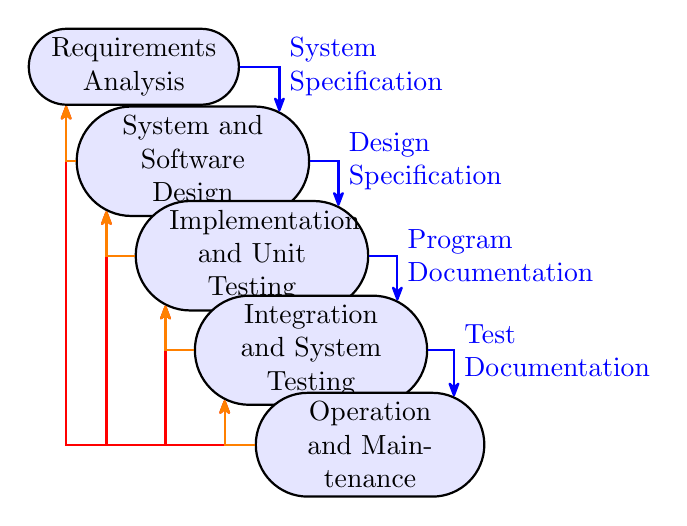
\begin{tikzpicture}[yscale=-1.2,xscale=.75,phase/.style={draw,thick,rounded rectangle,fill=blue!10,align=center,text width=21mm},label/.style={auto,bend right,align=left},to/.style={->,>={Stealth[round]},thick}]
			\node[phase,visible on=<6->] (1) at (0,0) {Requirements Analysis};
			\node[phase,visible on=<7->] (2) at (1,1) {System and Software Design};
			\node[phase,visible on=<2->] (3) at (2,2) {Implementation and Unit Testing};
			\node[phase,visible on=<4->] (4) at (3,3) {Integration and System Testing};
			\node[phase,visible on=<3->] (5) at (4,4) {Operation and Maintenance};
			\draw[to,visible on=<8->,blue] (1) -| node[label] {System\\Specification} (2.30);
			\draw[to,visible on=<8->,blue] (2) -| node[label] {Design\\Specification} (3.30);
			\draw[to,visible on=<5->,blue] (3) -| node[label] {Program\\Documentation} (4.30);
			\draw[to,visible on=<5->,blue] (4) -| node[label] {Test\\Documentation} (5.30);
			\draw[to,visible on=<9|handout:0>,red] (5) -| (1.210);
			\draw[to,visible on=<9|handout:0>,red] (5) -| (2.210);
			\draw[to,visible on=<9|handout:0>,red] (5) -| (3.210);
			\draw[to,visible on=<9|handout:0>,red] (5) -| (4.210);
			\draw[to,visible on=<10->,orange] (2) -| (1.210);
			\draw[to,visible on=<10->,orange] (3) -| (2.210);
			\draw[to,visible on=<10->,orange] (4) -| (3.210);
			\draw[to,visible on=<10->,orange] (5) -| (4.210);
	\end{tikzpicture}}
}

% introduced: process
% reused: ?
\newcommand{\diagramVModel}{
	{\color{black}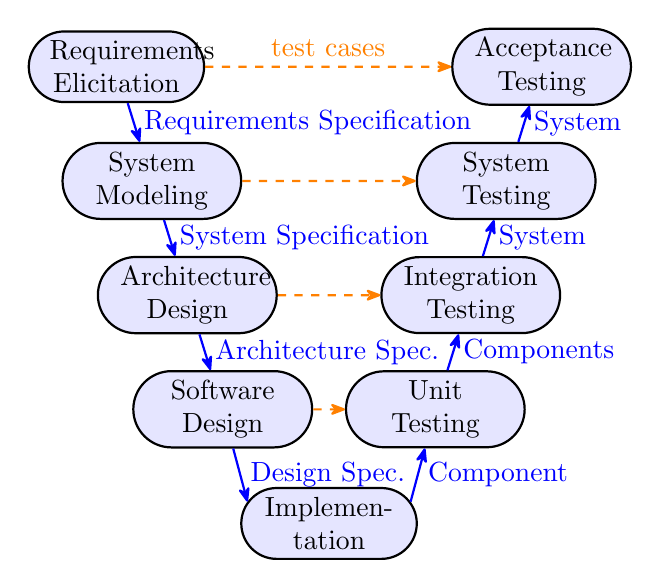
\begin{tikzpicture}[yscale=-1.45,xscale=.45,phase/.style={draw,thick,rounded rectangle,fill=blue!10,align=center,text width=17mm},label/.style={midway,anchor=west},to/.style={->,>={Stealth[round]},thick}]
			\node[phase,visible on=<2->] (1) at (0,0) {Requirements Elicitation};
			\node[phase,visible on=<3->] (2) at (1,1) {System Modeling};
			\node[phase,visible on=<4->] (3) at (2,2) {Architecture Design};
			\node[phase,visible on=<5->] (4) at (3,3) {Software Design};
			\node[phase,visible on=<6->] (5) at (6,4) {Implemen-tation};
			\node[phase,visible on=<7->] (6) at (9,3) {Unit\\Testing};
			\node[phase,visible on=<8->] (7) at (10,2) {Integration Testing};
			\node[phase,visible on=<9->] (8) at (11,1) {System Testing};
			\node[phase,visible on=<10->] (9) at (12,0) {Acceptance Testing};
			\draw[to,visible on=<3->,blue] (1) to node[label] {Requirements Specification} (2);
			\draw[to,visible on=<4->,blue] (2) to node[label] {System Specification} (3);
			\draw[to,visible on=<5->,blue] (3) to node[label] {Architecture Spec.} (4);
			\draw[to,visible on=<6->,blue] (4) to node[label] {Design Spec.} (5.165);
			\draw[to,visible on=<7->,blue] (5.15) to node[label] {Component} (6);
			\draw[to,visible on=<8->,blue] (6) to node[label] {Components} (7);
			\draw[to,visible on=<9->,blue] (7) to node[label] {System} (8);
			\draw[to,visible on=<10->,blue] (8) to node[label] {System} (9);
			\draw[to,visible on=<11->,orange,dashed] (1) to node[auto] {test cases} (9);
			\draw[to,visible on=<12->,orange,dashed] (2) to (8);
			\draw[to,visible on=<12->,orange,dashed] (3) to (7);
			\draw[to,visible on=<12->,orange,dashed] (4) to (6);
	\end{tikzpicture}}
}

% introduced: process
% reused: process
\newcommand{\diagramScrum}{
	\pic[width=\linewidth]{process/scrum}
}

% introduced: requirements
% reused: summary
\newcommand{\slideMindmapNonFunctionalRequirements}{
	{\newcommand{\requirements}{requirements}%
		\begin{tikzpicture}
			\path[%grow cyclic,
			small mindmap,
			%every node/.style=concept,
			concept color=green!20!background,
			%	text width=20mm,align=flush center,
			%	level 1/.append style={level distance=27mm,sibling angle=360/3},
			]
			node[concept] {non-functional \requirements}
			[counterclockwise from=195]
			child[concept color=blue!20!background] { node[concept] {product \requirements} 
				[counterclockwise from=75]
				child[visible on=<2->] { node[concept] {usability \requirements} }
				child[visible on=<3->] { node[concept] {efficiency \requirements} 
					[counterclockwise from=165]
					child { node[concept] {performance \requirements} }
					child { node[concept] {space \requirements} }
				}
				child[visible on=<4->] { node[concept] {dependability \requirements} }
				child[visible on=<5->] { node[concept] {security \requirements} }
			}
			child[concept color=red!20!background] { node[concept] {organizational \requirements} 
				[counterclockwise from=210]
				child[visible on=<6->] { node[concept] {environmental \requirements} }
				child[visible on=<7->] { node[concept] {operational \requirements} }
				child[visible on=<8->] { node[concept] {development \requirements} }
			}
			child[concept color=orange!20!background] { node[concept] {external \requirements} 
				[counterclockwise from=285]
				child[visible on=<9->] { node[concept] {regulatory \requirements} }
				child[visible on=<10->] { node[concept] {ethical \requirements} }
				child[visible on=<11->] { node[concept] {legislative \requirements}
					[counterclockwise from=-15]
					child { node[concept] {accounting \requirements} }
					child { node[concept] {safety/security \requirements} }
				}
			}
			;
	\end{tikzpicture}}
}

% introduced: modeling
% reused: architecture, design, summary
% 
% legend: gray (will not be taught), bold (taught in this lecture), normal font (will be taught)
% 02-requirements: use case diagrams
% 03-modeling: UML, activity diagrams, state machine diagrams
% 04-architecture: component diagrams
% 05-design: class diagrams, sequence diagrams
%
% parameters: use case, activity, state machine, component, class, sequence, structure, behavior, interactions
\tikzset{notTaughtUMLDiagrams/.style={text=gray}}
\newcommand{\slideMindmapUMLdiagrams}[9]{
	{\centering
		\begin{tikzpicture}
			\path[small mindmap,
			every node/.style={concept,font=\footnotesize},
			emph/.style={font=\bfseries\footnotesize},
			blue/.style={emph,text=blue},
			red/.style={emph,text=red},
			concept color=green!20!background,
			level 1/.append style={level distance=35mm,sibling angle=360/3},
			level 2/.append style={level distance=20mm,sibling angle=360/8},
			level 3/.append style={level distance=20mm,sibling angle=360/8},
			]
			node {UML Diagrams}
			[clockwise from=150]
			child[concept color=blue!20!background,#7] { node {Structure Diagrams} 
				[counterclockwise from=15]
				child { node[#4] {Component Diagram} }
				child { node[#5] {Class Diagram} }
				child[notTaughtUMLDiagrams] { node {Profile Diagram} }
				child[notTaughtUMLDiagrams] { node {Composite Structure Diagram} }
				child[notTaughtUMLDiagrams] { node {Deployment Diagram} }
				child[notTaughtUMLDiagrams] { node {Object Diagram} }
				child[notTaughtUMLDiagrams] { node {Package Diagram} }
			}
			child[concept color=red!20!background,#8] { node {Behavior Diagrams} 
				[clockwise from=135]
				child { node[#1] {Use Case Diagram} }
				child { node[#2] {Activity Diagram} }
				child { node[#3] {State Machine Diagram} }
				child[concept color=orange!20!background,#9] { node {Interaction Diagrams} 
					[clockwise from=30]
					child { node[#6] {Sequence Diagram} }
					child[notTaughtUMLDiagrams] { node {Communi-cation Diagram} }
					child[notTaughtUMLDiagrams] { node {Interaction Overview Diagram} }
					child[notTaughtUMLDiagrams] { node {Timing Diagram} }
				}
			}
			;
	\end{tikzpicture}}
}

% introduced: architecture
% reused: summary
\newcommand{\slideArchitecturalPattern}{
	\begin{fancycolumns}
		\centering
		\begin{definition}{Architectural Pattern\mysource{\sommerville}}
			\mycite{Architectural patterns capture the essence of an architecture that has been used in different software systems. [...] Architectural patterns are a means of reusing knowledge about generic system architectures.}
		\end{definition}
		\nextcolumn
		\begin{note}{Goals}
			\partofpage{35}{
				\pic[width=\textwidth]{database}
			}
			\partofpage{60}{
				\begin{itemize}
					\item preserve knowledge of software architects
					\item reuse of established architectures
					\item enable efficient communication
				\end{itemize}
			}
		\end{note}
	\end{fancycolumns}
}

% introduced: architecture
% reused: compilation?
\newcommand{\slidePipeAndFilter}{
	\begin{fancycolumns}[animation=none]
		\begin{definition}{Pipe-and-Filter Architecture \mysource{\sommerville}}
			\begin{itemize}
				\item \emph{Problem}: data is processed in numerous processing steps, which are prone to change
				\item \emph{Idea}: modularization of each processing step into a component
				\item filter components process a stream of data continously
				\item pipes transfer data unchanged from filter output to filter input
			\end{itemize}
		\end{definition}
		\uncover<2->{
			\begin{example}{Pipe Operator in UNIX}
				\mycite{\texttt{ls -al | grep '2020' | grep -v 'Nov' | more}} searches files in a folder from the year 2020 except those from November and delivers the results in pages.
			\end{example}
		}
		\nextcolumn%
		\uncover<3->{\hfill\href{https://commons.wikimedia.org/wiki/File:Pipeline-notitle.svg}{\picDark[width=.8\textwidth]{pipe-and-filter}}}%
	\end{fancycolumns}
}

% introduced: reuse
% reused: summary
%
% legend: gray (will not be taught), bold (taught in this lecture), normal font (will be taught)
% 
% parameters: object adapter, composite, decorator, singleton, abstract factory, observer, structural, creational, behavioral
\tikzset{notTaughtDesignPatterns/.style={text=gray}}
\newcommand{\slideMindmapDesignPatterns}[9]{
	{\centering
		\begin{tikzpicture}
			\path[small mindmap,
			every node/.style={concept,font=\scriptsize},
			emph/.style={font=\bfseries\scriptsize},
			blue/.style={emph,text=blue},
			red/.style={emph,text=red},
			concept color=green!20!background,
			level 1/.append style={level distance=35mm,sibling angle=65},
			level 2/.append style={level distance=20mm,sibling angle=360/12},
			level 3/.append style={level distance=20mm,sibling angle=360/8},
			]
			node {Design Patterns}
			[clockwise from=155]
			child[concept color=blue!20!background,#7] { node {Structural Patterns} 
				[clockwise from=215]
				child[#1] { node {Object Adapter} }
				child[notTaughtDesignPatterns] { node {Class Adapter} }
				child[notTaughtDesignPatterns] { node {Bridge} }
				child[#2] { node {Composite} }
				child[#3] { node {Decorator} }
				child[notTaughtDesignPatterns] { node {Facade} }
				child[notTaughtDesignPatterns] { node {Flyweight} }
				child[notTaughtDesignPatterns] { node {Proxy} }
			}
			child[concept color=red!20!background,#8] { node {Creational Patterns} 
				[clockwise from=150]
				child[#5] { node {Abstract Factory} }
				child[notTaughtDesignPatterns] { node {Builder} }
				child[notTaughtDesignPatterns] { node {Factory Method} }
				child[notTaughtDesignPatterns] { node {Prototype} }
				child[#4] { node {Singleton} }
			}
			child[concept color=orange!20!background,#9] { node {Behavioral Patterns} 
				[clockwise from=175]
				child[notTaughtDesignPatterns] { node {Chain of Responsibility} }
				child[notTaughtDesignPatterns] { node {Command} }
				child[notTaughtDesignPatterns] { node {Interpreter} }
				child[notTaughtDesignPatterns] { node {Iterator} }
				child[notTaughtDesignPatterns] { node {Mediator} }
				child[notTaughtDesignPatterns] { node {Memento} }
				child[#6] { node {Observer} }
				child[notTaughtDesignPatterns] { node {State} }
				child[notTaughtDesignPatterns] { node {Strategy} }
				child[notTaughtDesignPatterns] { node {Template Method} }
				child[notTaughtDesignPatterns] { node {Visitor} }
			}
			;
	\end{tikzpicture}}
}



% HOPEFULLY NON-PERMANENT HACKS

\usepackage{pgf, tikz}
\usetikzlibrary{arrows, arrows.meta, positioning, shapes, calc, decorations.text, shadows.blur, matrix, fit, mindmap, backgrounds}
\tikzset{ >=stealth'} % define standard arrow tip
\usepackage{tikz-qtree}

\newcommand{\handoutonly}[1]{}
\newcommand{\slideonly}[1]{#1}
\mode<handout>{
	\renewcommand{\handoutonly}[1]{#1}
	\renewcommand{\slideonly}[1]{}
}
\newcommand{\prehandout}[1]{#1}
\newcommand{\posthandout}[1]{}

% Keys to support piece-wise uncovering of elements in TikZ pictures:
% \node[visible on=<2->](foo){Foo}
% \node[visible on=<{2,4}>](bar){Bar}   % put braces around comma expressions
%
% Internally works by setting opacity=0 when invisible, which has the 
% adavantage (compared to \node<2->(foo){Foo} that the node is always there, hence
% always consumes space plus that coordinate (foo) is always available.
%
% The actual command that implements the invisibility can be overriden
% by altering the style invisible. For instance \tikzsset{invisible/.style={opacity=0.2}}
% would dim the "invisible" parts. Alternatively, the color might be set to white, if the
% output driver does not support transparencies (e.g., PS) 
%
\tikzset{
	invisible/.style={opacity=0},
	visible on/.style={alt={#1{}{invisible}}},
	alt/.code args={<#1>#2#3}{%
		\alt<#1>{\pgfkeysalso{#2}}{\pgfkeysalso{#3}} % \pgfkeysalso doesn't change the path
	},
}

\usepackage{tabularx}
